
\subsection*{Probability Distribution Types}

Probability distributions are mathematical functions that describe the likelihood of different outcomes. These distributions provide the mathematical basis for modeling uncertainties and variability in complex systems. Below is a concise summary that contrasts the key characteristics, probability density functions (PDFs), and common uses of several fundamental distributions. This comparison facilitates a deeper understanding of when and why each distribution type might be applied in practical scenarios.

\begin{table}[ht]
\centering
\caption{Summary of Different Probability Distributions}
\begin{tabular}{|l|l|l|l|}
\hline
\textbf{Distribution} & \textbf{Characteristics} & \textbf{PDF Formula} & \textbf{Common Uses} \\
\hline
Normal & Symmetrical, bell-shaped & \(f(x) = \frac{1}{\sigma\sqrt{2\pi}} e^{-\frac{1}{2}\left(\frac{x-\mu}{\sigma}\right)^2}\) & Error measurement \\
\hline
Log-Normal & Right-skewed & \(f(x) = \frac{1}{x\sigma\sqrt{2\pi}} e^{-\frac{(\ln x - \mu)^2}{2\sigma^2}}\) & Financial modeling \\
\hline
Exponential & Constant hazard rate & \(f(x;\lambda) = \lambda e^{-\lambda x}\) & Time until event \\
\hline
Binomial & Fixed number of trials & \(P(X=k) = \binom{n}{k} p^k (1-p)^{n-k}\) & Success count in trials \\
\hline
Poisson & Events in fixed interval & \(P(X=k) = \frac{\lambda^k e^{-\lambda}}{k!}\) & Counting rare events \\
\hline
\end{tabular}
\label{table:distributions}
\end{table}

\begin{figure}[ht]
\centering
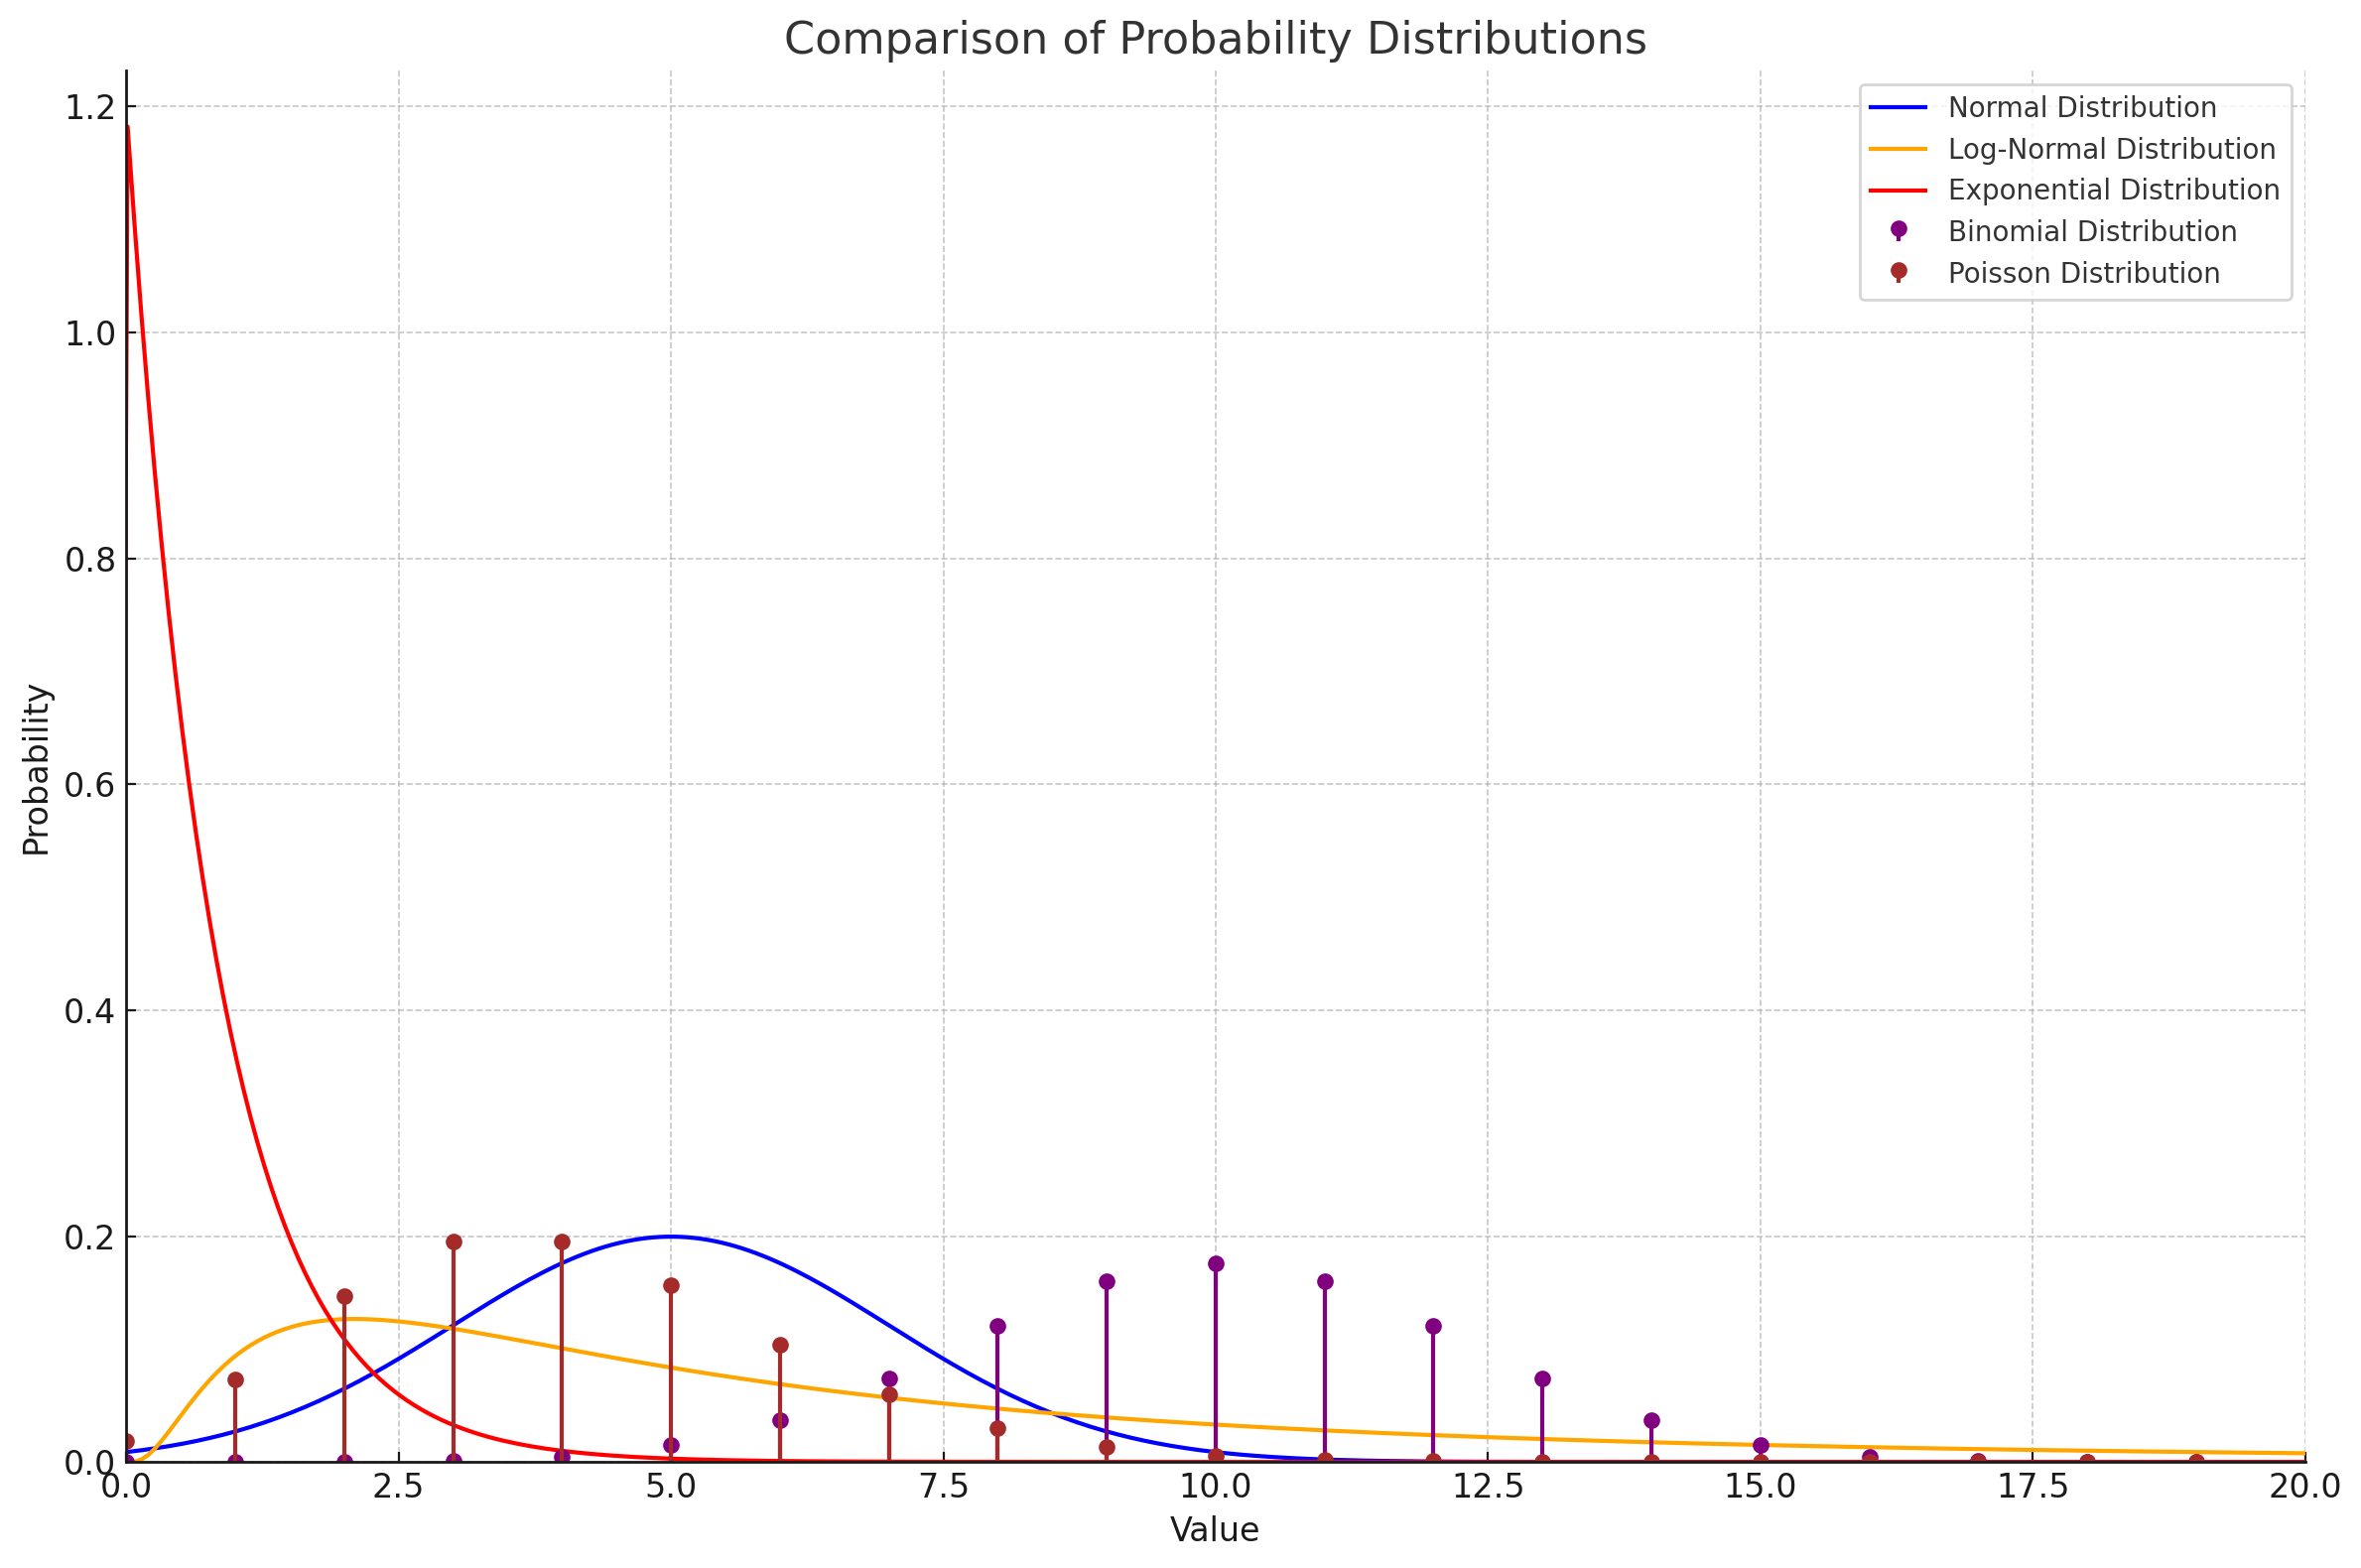
\includegraphics[width=0.8\linewidth]{figures/dis.png}
\caption{Comparative visualization of different probability distributions. The distributions are parameterized as follows: Normal Distribution with mean (\( \mu = 5 \)) and standard deviation (\( \sigma = 2 \)); Log-Normal Distribution with shape (\( \sigma = 0.954 \)) and scale (\( e^{1.65} \)); Exponential Distribution with the rate (\( \lambda = 1.2 \)); Binomial Distribution with number of trials (\( n = 20 \)) and probability of success (\( p = 0.5 \)); Poisson Distribution with the average rate (\( \lambda = 4 \)). These parameters offer a glimpse into the diverse behaviors of distributions across a range of disciplines, from engineering to economics.}
\label{fig:distributions}
\end{figure}



\subsubsection*{Normal Distribution}

The Normal Distribution occurs naturally in many physical, biological, and social processes. Its symmetric, bell-shaped curve represents the distribution of variables influenced by numerous small, random disturbances. 
\begin{mdframed}

The \textbf{Central Limit Theorem} underpins its significance, suggesting that sums of independent random variables tend toward a normal distribution, irrespective of the original distribution shape.
\end{mdframed}

\begin{itemize}
    \item \textbf{Characteristics}: Central to the normal distribution are its mean (\( \mu \)), dictating the curve's center, and standard deviation (\( \sigma \)), controlling its spread. The total area under the curve corresponds to a probability of 1, reflecting the exhaustive outcomes.
    \item \textbf{Applications}: Its applications span from quantifying measurement errors to modeling uncertainties in engineering and finance. 
    \item \textbf{Example Problem}: An example involves estimating probabilities related to the mean height within a population, assuming heights are normally distributed.
\end{itemize}


\subsubsection*{Log-Normal Distribution}

The Log-Normal Distribution models variables that are the product of many independent, positive random variables. It is skewed right and suitable for representing quantities like income, where values are positive and can span several orders of magnitude.

\begin{itemize}
    \item \textbf{Characteristics}: It is defined for \(x > 0\) with parameters \(\mu\) and \(\sigma\), representing the mean and standard deviation of the variable's natural logarithm. 
    \item \textbf{Applications}: From modeling stock prices to material strengths, the log-normal distribution aids in areas where growth processes or multiplicative effects are observed.
\end{itemize}

\subsubsection*{Exponential Distribution}

The Exponential Distribution is often used to model the time between independent events that happen at a constant average rate. Its memorylessness property makes it essential for studying waiting times and system reliability.


\begin{itemize}
    \item \textbf{Characteristics}: It has a single parameter \( \lambda \), the rate at which events occur. The mean and standard deviation are both \(1/\lambda\).
    \item \textbf{Applications}: Widely used in survival analysis, queuing theory, and reliability engineering to model the time until an event, such as system failure, occurs.
\end{itemize}

\subsubsection*{Binomial Distribution}

The Binomial Distribution models the number of successes in a fixed number of independent trials, each with two possible outcomes (success or failure) and a constant probability of success. 

The essence of the Binomial Distribution lies in its discrete nature, making it ideal for scenarios with a finite number of trials. It is the basis for the binomial test of statistical significance.


\begin{itemize}
    \item \textbf{Characteristics}: Defined by two parameters: the number of trials (\(n\)) and the probability of success (\(p\)) in each trial. The distribution is discrete, with the probability mass function giving the probability of achieving exactly \(k\) successes in \(n\) trials.
    \item \textbf{Applications}: Used in quality control, election predictions, and any scenario where the outcome follows a "success" or "failure" pattern, such as flipping coins or manufacturing defects.
    \item \textbf{Example Problem}: Determining the likelihood of getting exactly 10 heads in 20 flips of a fair coin.
\end{itemize}

\subsubsection*{Poisson Distribution}

The Poisson Distribution is a discrete probability distribution that expresses the probability of a given number of events occurring in a fixed interval of time or space if these events occur with a known constant mean rate and independently of the time since the last event.

It is particularly useful for modeling the number of events in fixed intervals of time or space, assuming that these events occur at a known constant rate and independently of each other.


\begin{itemize}
    \item \textbf{Characteristics}: Characterized by its single parameter (\(\lambda\)), the average rate of occurrence of the event per interval. The distribution predicts the probability of a number of events occurring in a fixed period.
    \item \textbf{Applications}: Essential for queueing theory, telecommunications, and traffic flow analysis, including modeling the number of calls received by a call center in an hour or the number of decay events from a radioactive source.
    \item \textbf{Example Problem}: Estimating the number of cars passing through a toll booth in an hour, given the average traffic flow rate.
\end{itemize}

\subsection*{Joint Probability Distributions}

Understanding the joint behavior of two or more stochastic variables is fundamental in fields such as finance, engineering, and environmental science. Joint probability distributions offer insights into how variables can simultaneously assume specific values, highlighting their collective behavior rather than isolated occurrences.


\begin{itemize}
    \item \textbf{Definition}: A joint probability distribution for variables \(X\) and \(Y\) quantifies the likelihood of both variables simultaneously falling within specific ranges or categories.
    \item \textbf{Independence vs. Dependence}: Independent variables' joint distribution can be constructed from the product of their individual distributions. However, dependencies between variables necessitate a more nuanced approach to accurately capture their joint behavior.
    \item \textbf{Exploring Relationships}: Measures such as covariance and correlation are critical in assessing the relationship between variables, offering insights into their directional and strength dynamics.
\end{itemize}

\subsubsection*{Did you know? - \href{http://www.tylervigen.com/spurious-correlations}{Correlation vs Causation}}
\begin{mdframed}[backgroundcolor=gray!20] 
It is essential to understand that correlation does not imply causation. Two variables may be correlated (i.e., they show a statistical relationship) without one causing the other. This distinction is crucial in data analysis and interpretation.
\end{mdframed} 

\begin{figure}
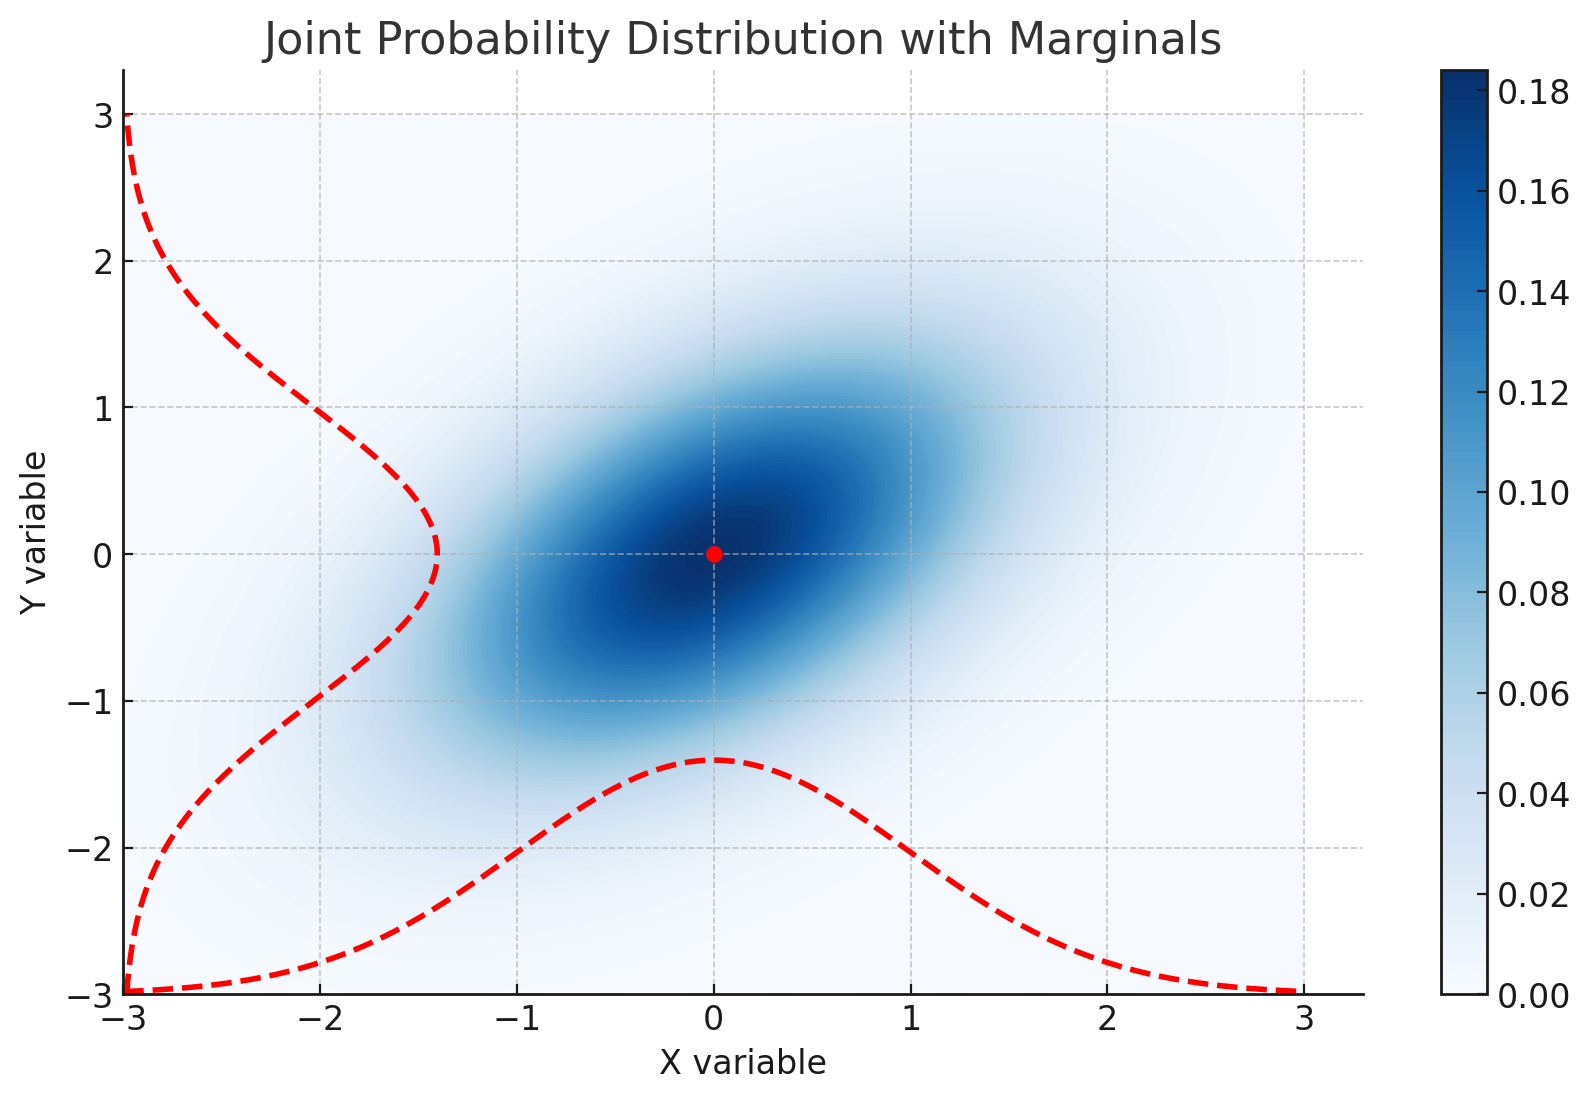
\includegraphics[width=\linewidth]{figures/2dis.png}
\caption{Joint Probability Distribution with Marginals. The dashed red lines represent the marginal distributions of X and Y, intersecting at the mean, the point of highest probability.}
\label{fig:distributions}
\end{figure}


\subsubsection*{Applications}
Joint distributions are pivotal in risk assessment, where understanding the interaction between different risk factors is essential for predicting the occurrence and impact of potential adverse events.

\subsection*{Extreme Value Distributions}

Extreme Value Distributions are pivotal in assessing the behavior of data at its extremes, rather than focusing on the mean or median. This analysis is crucial in domains such as environmental science, finance, and engineering, where the most extreme events, though rare, can have significant implications.

\subsubsection*{Generalized Extreme Value (GEV) Distribution}
The GEV distribution encompasses three distinct types of extreme value distributions: Gumbel, Fréchet, and Reverse Weibull. Each is suited to modeling different kinds of extreme event data, unified under a single framework characterized by location (\( \mu \)), scale (\( \sigma \)), and shape (\( \xi \)) parameters. The GEV distribution's flexibility makes it a cornerstone for extreme value theory, allowing for comprehensive modeling of tail behavior.

\[
G(x; \mu, \sigma, \xi) = 
\begin{cases} 
\exp\left(-\left[1 + \xi\left(\frac{x - \mu}{\sigma}\right)\right]^{-1/\xi}\right), & \xi \neq 0 \\
\exp\left(-\exp\left(-\frac{x - \mu}{\sigma}\right)\right), & \xi = 0 
\end{cases}
\]


\textit{Gumbel Distribution} (\( \xi = 0 \)): Suitable for data where extremes are near the central tendency. Used in environmental studies and climate modeling.
        \[ G(x; \mu, \sigma) = \exp\left(-\exp\left(-\frac{x - \mu}{\sigma}\right)\right) \]
\textit{Reverse Weibull Distribution} (\( \xi < 0 \)): Models data with a bounded maximum. Applied in material strength analysis and durability studies.
        \[ W(x; \mu, \sigma) = \exp\left(-\left(-\frac{x - \mu}{\sigma}\right)^\beta\right) \]
\textit{Fréchet Distribution} (\( \xi > 0 \)): Captures behavior of datasets with heavy tails. Commonly used in financial risk modeling.
        \[ F(x; \mu, \sigma, \alpha) = \exp\left(-\left(\frac{x - \mu}{\sigma}\right)^{-\alpha}\right) \]


\subsubsection*{Transformation from Uniform PDF to Extreme Value Distribution}
A fundamental technique in statistical modeling, the probability integral transform, is used to transform a uniform PDF to an extreme value distribution.

\paragraph{Step-by-Step Algorithm:}
\begin{enumerate}
    \item \textbf{Start with the Uniform Distribution CDF:} The CDF for a uniform distribution \(U(0, 1)\) is \(F_U(x) = x\), where \(0 \leq x \leq 1\).
    \[ F_U(x) = x \]
    \item \textbf{Apply the Inverse CDF of the GEV Distribution:} To transform this to a GEV distribution, the inverse CDF (Quantile function) of the GEV, \(G^{-1}(y; \mu, \sigma, \xi)\), is used, where \(y = F_U(x)\).
    \[ Y = G^{-1}(F_U(x); \mu, \sigma, \xi) \]
    \item \textbf{Resulting Transformation:} The transformed variable \(Y\) follows the GEV distribution with specified parameters.
\end{enumerate}

\subsubsection*{Fisher-Tippett-Gnedenko Theorem}
This theorem underpins the use of extreme value distributions, stating that the limit distribution of the normalized maxima (or minima) of a sequence of independent, identically distributed random variables falls into one of the extreme value distribution types. It justifies the application of these distributions in modeling and predicting extreme events across various fields.


\subsubsection*{Applications and Selection Criteria}

\begin{table}[ht]
\centering
\caption{Parent Distributions and Their Corresponding Asymptotic Extreme Value Types}
\begin{tabular}{|p{3cm}|p{4cm}|p{3cm}|p{3cm}|}
\hline
\textbf{Parent Distribution} & \textbf{Domain of Attraction} & \textbf{Examples} & \textbf{Applications} \\
\hline
Uniform, Beta (Short tail) & Reverse Weibull & Hydrological data, Material strength & Structures under stress, Durability \\
\hline
Normal, Exponential, Gamma, Lognormal, Weibull (Light tail) & Gumbel & Environmental data, Operational lifetimes & Climate modeling, Reliability engineering \\
\hline
Pareto, Cauchy, Student-t (Fat tail) & Fréchet & Financial returns, Catastrophic events & Financial risk, Natural disaster analysis \\
\hline
\end{tabular}
\label{table:GEV_domain_of_attraction}
\end{table}

This tabular representation aids in determining the appropriate extreme value distribution for a given set of data by relating it back to its parent distribution, highlighting the importance

\subsection*{Assignment 2: Exponential Distribution and Pollution Events}
This assignment explores the practical application of exponential distributions in environmental engineering. It focuses on the probability of pollution events exceeding a critical threshold.

It requires understanding the exponential distribution's role in modeling time between events. Think of:

\begin{itemize}
    \item A distribution known for its memoryless property and how this characteristic informs environmental risk evaluation.
    \item Reflecting on the significance of certain distribution features that allow us to interpret and forecast event frequencies within a given context.
    \item Utilizing simulation techniques to approximate real-world variability and assess the robustness of statistical predictions.
\end{itemize}

The challenge posed by this assignment emphasizes the synthesis of theoretical knowledge with practical data analysis skills, particularly in constructing and interpreting probabilistic models that describe environmental phenomena.

\subsection*{Assignment 3: From Uniformity to Extremes}
This assignment introduces the concept of extreme values derived from uniform distributions, focusing on the behavior of maximum values within a dataset. You have to link an understanding of uniform distributions with the concept of extreme value theory. Consider

\begin{itemize}
    \item The exploration of uniformity in data and its transformation under extreme conditions, highlighting the broader implications of distributional assumptions.
    \item The application of graphical techniques to interpret the distribution of data points, an exercise that sharpens analytical visualization skills.
    \item The use of a theoretical framework to comprehend the behavior of data at its limits and the role this plays in predictive modeling.
\end{itemize}